\documentclass[a4,center,fleqn]{NAR}

% Enter dates of publication
\copyrightyear{2015}
\pubdate{31 July 2016}
\pubyear{2016}
\jvolume{37}
\jissue{12}

%\articlesubtype{This is the article type (optional)}

\begin{document}

\title{USR@istar: a large-scale ligand-based virtual screening webserver using ultrafast shape recognition methods}

\author{
Hongjian Li\,$^{1}$,
Kwong-Sak Leung\,$^{1}$,
Man-Hon Wong\,$^{1}$
and Pedro J. Ballester\,$^{2}$
\footnote{To whom correspondence should be addressed.
Tel: +33-486-977-265; Fax: +33-486-977-499; Email: pedro.ballester@inserm.fr}}

\address{
$^{1}$Department of Computer Science and Engineering, Chinese University of Hong Kong, Sha Tin, New Territories, Hong Kong
and
$^{2}$Cancer Research Center of Marseille, INSERM U1068, F-13009, Marseille, France. Institut Paoli-Calmettes, F-13009, Marseille, France. Aix-Marseille Université, F-13284, Marseille, France. CNRS UMR7258, F-13009, Marseille, France.}
% Affiliation must include:
% Department name, institution name, full road and district address,
% state, Zip or postal code, country

\history{
Received January 1, 2015;
Revised February 1, 2016;
Accepted March 1, 2016}

\maketitle

\begin{abstract}

Finding compounds geometrically and structurally similar to a query molecule has been an important but daunting problem for a long time. The USR (Ultrafast Shape Recognition) algorithm represents a whole new alignment-free method that encodes the shape information semantically and permits superfast screening of a large molecular database. Several extensions to USR improve the original method from various perspectives and three of them, UFSRAT, EDULISS and SwissTargetPrediction, are also available as web servers. However, UFSRAT and EDULISS are unable to discriminate between long, chain-like molecules, and their calculated distributions are not meaningful when some pharmacophoric features are rarer than others. SwissTargetPrediction uses a small, well annotated, bioactive compound database and is generally for target fishing.

For prospective virtual screening purposes, in this study we have implemented USR and its extension USRCAT (USR with Credo Atom Types) on top of our istar web platform. We used a large molecular library consisting of 23,129,049 diverse compounds collected from the ZINC database, and generated 1,737,652,473 diverse conformers. We exploited three levels of parallelism, and implemented a fast and novel method to compute sum of absolute differences using AVX (Advanced Vector Extensions) to accelerate similarity score calculation. Our USR@istar supports query molecules in SDF format, and interfaces with our iview WebGL visualizer for interactive visualization of high-score hits. USR@istar is freely available at http://istar.cse.cuhk.edu.hk/usr.

To thoroughly benchmark USR@istar, we selected 19 query molecules with different molecular sizes. Not unexpectedly, ranking by USR or USRCAT score yielded different output, particularly if the query molecule was large. When the query molecule had more than four rotatable bonds, both methods failed to recover the query molecule in a different pose in the output due to the large torsional diversity implied. Surprisingly, input file format was found to affect the classification of atoms into predefined pharmacophoric subsets. We also observed that loading database features in advance significantly reduced the matching runtime from 167 seconds to just 30 seconds on average for a query.

\end{abstract}

% **************************************************************
% Keep this command to avoid text of first page running into the
% first page footnotes
\enlargethispage{-65.1pt}
% **************************************************************

\section{Introduction}

Molecular shape has been widely acknowledged as a key factor for biological activity and is thus regarded as a very important pattern for drug searching. Searching a molecular database for compounds that most closely resemble the shape of a given query molecule, be it a known inhibitor of a target protein, a natural product, or even a patented compound, finds pragmatic applications in ligand-based virtual screening \cite{1332,1380,1281,1504,1502,1615} and target fishing \cite{1528,1407,1408,1402}. Therefore molecular similarity search can assist in discovering structurally novel active compounds, or in identifying potential interacting target of bioactive ligands, which is useful for understanding the polypharmacology and safety profile of existing drugs. Furthermore, this approach can be applied to other scientific disciplines such as performing similarity comparisons between proteins or designing content-based Internet search engines for 3D geometrical objects \cite{1280}.

Molecular shape similarity can be quantified by methods based on structural alignment \cite{1440,887,1439,1534} or shape recognition \cite{1379,1338,1331,1675}. Structural alignment is also known as molecular superposition, and requires precise geometric comparison, which is often computationally demanding. Shape recognition, on the other hand, encodes shape information into a numerical feature vector, which can be subsequently used to compute a similarity score between two molecules very efficiently.

USR (Ultrafast Shape Recognition) \cite{1379} was the first non-superposition method for molecular shape comparison, and demonstrated superior computational performance at least three orders of magnitude faster than previously existing alignment-based methods. USR has another major advantage of being invariant to spatial rotation and translation, and hence circumvents the problematic requirement of aligning molecules. USR defines the shape of a molecule independently and for every molecule uses a fixed set of 12 descriptors derived from the first 3 statistical moments of distributions of interatomic distances between atoms and 4 purposely-selected centroids. This encoding scheme ensures that every molecule has a unique location in the 12-dimensional chemical space spanned by the used descriptors, and consequently enables finding and visualizing clusters of molecules with similar shapes \cite{1280,1332}. Selecting the most representative molecule of each cluster can avoid repeating expensive biological tests on similar molecules \cite{1280}. The ability of USR as a standalone method was studied to identify molecules sharing common biological activities through retrospective \cite{1332} and prospective \cite{1380,1281,1504,1502,1615} virtual screening experiments. Prospectively, USR was applied to the discovery of inhibitors of arylamine NATs (N-acetyltransferases) \cite{1380}, DHQase2 (dehydroquinase type 2) \cite{1281}, PAD4 (protein arginine deiminase type 4) \cite{1504}, p53-MDM2 (murine double minute 2) \cite{1502}, and PRL-3 (phosphatase of regenerating liver) \cite{1615}. USR was also used for deduplication in a virtual screening campaign \cite{1390} and in our iSyn \cite{1409,1387} \textit{de novo} ligand design software.

Since USR was devised in 2007, there have been quite a few extensions \cite{1333,1436,1437,1334,1335,1337,1338,1331,1407,1408,1675} to augment the original method. \cite{1333} presented a hybrid approach composed of USR and the topological MACCS key descriptors, which are binary in nature and encode the presence or absence of 166 predefined structural fragments. It used the first four unbalanced moments of each distribution of atomic distances and incorporated additional chemical information through 2D structural similarity. Random Forest \cite{1309} was used for multi-class classification. Incorporating an additional central moment, the kurtosis, was found to significantly improve the performance. The addition of the fifth central moment, however, did not improve the performance sufficiently to justify the increased computational expense.

UFSRAT \cite{1436} addressed the lack of discrimination between compounds having similar shape but distinct pharmacophoric features by subdividing atoms into four subsets which are heavy, hydrophobic, hydrogen bond acceptor or donor atoms, according to their atom types. For each subset, the four centroids were calculated, and so were the 12 USR descriptors. Therefore 48 descriptors were resulted. This was to ensure that similar compounds are able to make the same type of interactions within biological systems as the query molecule. UFSRAT was prospectively applied to the discovery of inhibitors of 11$\beta$-HSD1 (hydroxysteroid dehydrogenase type 1) \cite{1505}. UFSRAT is available as a web server at http://opus.bch.ed.ac.uk/ufsrat/, which contains 28 databases with the largest one containing 4,853,000 conformers. UFSRAT is also employed for geometrical similarity searches in the EDULISS database \cite{1437} available at http://eduliss.bch.ed.ac.uk/, which comprises over 5 million commercially available compounds.

CSR \cite{1334} and USR:OptIso \cite{1335} attempted to tackle the lack of discrimination between chiral compounds. Their novel idea was to position the centroids in such a way that they clearly distinguish between enantiomers, i.e. optical isomers. They both used cross product because it is an operator that transforms equivariantly under rotations and translations, but not under reflections. The two methods differed in selecting the centroids and in replacing or supplementing the new optical isomerism descriptor \cite{1335}. CSR \cite{1334} was tested on the DUD (Directory of Decoys) dataset \cite{87}, where a significant improvement in enrichment was found over USR. USR:OptIso \cite{1335} was shown to be helpful for analyzing molecules with stereogenic centers, atropisomerism, and in the clustering of conformers generated by systematic bond rotation.

ElectroShape \cite{1337,1338} extended the CSR \cite{1334} method by encoding electrostatics and liphophilicity through additional dimensions and centroids. In \cite{1337}, the partial charge was represented as a fourth coordinate, with atoms being identified by points in four-dimensional space. ElectroShape was validated using release 2 of the DUD dataset \cite{87}, and showed a near doubling in enrichment over USR and CSR. Different implementations of partial charge were also revealed to affect the enrichment performance significantly. The addition of a fourth statistical moment, as was done in \cite{1333}, improved USR and CSR but not ElectroShape, suggesting that adding extra information might not necessarily improve enrichment but could dilute the information already included. In \cite{1338}, ElectroShape was further extended by using atomic lipophilicity as an additional molecular property, with atoms being identified by points in five-dimensional space. This version of ElectroShape showed a clear improvement in performance, indicating that adding extra independent atomic properties makes shape-based enrichments even better.

USRCAT \cite{1331} extended the UFSRAT \cite{1436} method by identifying five pharmacophoric subsets of atoms with the help of the SMARTS patterns used for atom typing in the CREDO database \cite{522,1530}. The five subsets were chosen to be heavy, hydrophobic, aromatic, hydrogen bond acceptor or donor atoms. Aromaticity was added to USRCAT as a pharmacophoric subset because USR was unable to discriminate between long, chain-like molecules such as certain heteropeptides and long alkylchains in particular. Unlike UFSRAT \cite{1436}, USRCAT \cite{1331} derived the four centroids from heavy atom coordinates and used them to calculate the distributions for all the five subset moments to improve screening performance. USRCAT was shown to outperform the traditional USR method in a retrospective virtual screening benchmark on the DUD-E (Directory of Decoys, Enhanced) dataset \cite{1185}. The highest enrichment factors were only achieved if the LEC (Lowest Energy Conformer) of an active was used as a query and if the LECs were included in the target set, but this observation could not be generalized. DUD-E was found to be not ideal to benchmark the virtual screening performance of global shape similarity algorithms such as USR and its variants due to the large variations in molecular size of the active ligands. Another extension TopMap \cite{1675} adopted a similar idea but partitioned the molecular coordinates into different charge-tiers and used five descriptors of the shape distributions to construct a feature vector.

A recent study \cite{1407} used a reference set of 224,412 molecules active on 1,700 human proteins and showed that accurate target prediction can be achieved by using a multiple logistic regression to combine different measures of chemical similarity based on both chemical structure and molecular shape, with the former using FP2 fingerprints and the latter using ElectroShape \cite{1338}. This hybrid method was subsequently encapsulated into the SwissTargetPrediction \cite{1408} web server, freely available at http://www.swisstargetprediction.ch/, to identify new targets for uncharacterized molecules or secondary targets for known molecules. With data collected from the ChEMBL database version 16 \cite{1441}, the molecular library was expanded to 280,000 compounds active on 2,686 targets of the organisms of human, mouse, rat, cow and horse. Mapping predictions by homology within and between different species, a powerful approach to translate results obtained in model organisms to human, were enabled for close paralogs and orthologs.

Table \ref{Methods} summarizes USR and its variants.

\begin{table*}
\tableparts{
\caption{Summary of USR-like methods.}
\label{Methods}
}{
\begin{tabular*}{\columnwidth}{@{}lll@{}}
\toprule
method & novelty & references\\
\colrule
USR          & encoding shape by atomic distribution & \cite{1379}\\
USR+MACCS    & incorporating chemical similarity     & \cite{1333}\\
UFSRAT       & subdiving atoms into subsets          & \cite{1436,1437}\\
CSR          & repositioning reference locations     & \cite{1334}\\
USR:OptIso   & repositioning reference locations     & \cite{1335}\\
ElectroShape & expanding coordinate dimension        & \cite{1337,1338}\\
USRCAT       & subdiving atoms into subsets          & \cite{1331}\\
TopMap       & subdiving atoms into subsets          & \cite{1675}\\
SwissTargetPrediction & mixing ElectroShape and chemical similarity & \cite{1407,1408}\\
\botrule
\end{tabular*}
}
{}%This is a table footnote
\end{table*}

Among the USR variants mentioned above, only three of them \cite{1436,1437,1408} have been made available as web servers together with different databases for different purposes. The UFSRAT \cite{1436} and EDULISS \cite{1437} web servers both employ the UFSRAT \cite{1436} method for ligand similarity search. However, as pointed out in \cite{1331}, this method is incapable of discriminating between long, chain-like molecules such as certain heteropeptides and long alkylchains because aromaticity is not considered as a pharmacophoric subset; besides, calculating the four centroids for each set of atoms individually is problematic because either the parameters cannot be calculated at all or the underlying distance distributions are not with respect to the overall shape of a molecule and not meaningful when some pharmacophoric features are rarer than others. The UFSRAT \cite{1436} web server restricts the input query molecule to be one molecule in SDF format only, and does not support online visualization. The EDULISS \cite{1437} web server requires drawing a query structure in a Java molecular editor, which is being disabled on more and more systems due to security concerns. The SwissTargetPrediction \cite{1408} web server, on the other hand, comprises well-annotated active compounds and is primarily used for predicting the target proteins of bioactive small molecules but not for prospective virtual screening purposes.

In this project we aimed to provide an istar-based \cite{1362} web service for large-scale prospective virtual screening using USR-like methods. We chose to employ USR \cite{1379} and USRCAT \cite{1331} because they have demonstrated pragmatic usefulness in prospective \cite{1380,1281,1504,1502,1615} and retrospective \cite{1331} virtual screening experiments, respectively, and their Python source code is freely available for studying the precise implementation and porting to other programming languages such as C++ and JavaScript.

Our USR@istar has several distinct features. First, it uses both USR and USRCAT to search a large database comprising 23 million compounds collected from ZINC \cite{532,1178}. Second, it utilizes three levels of parallelism, both coarse grained and fine grained, to accelerate job execution. Third, it interfaces with the iview \cite{1366} WebGL visualizer to display results in an interactive manner.

\section{MATERIALS AND METHODS}

This section first reviews the general methods of USR \cite{1379} and USRCAT \cite{1331}, and then introduces their specific implementations on our istar platform \cite{1362}.

\subsection{USR and USRCAT}

USR is based on the observation that the shape of a molecule is uniquely determined by the relative position of its atoms, which is in turn determined by the set of all interatomic distances. This convenient representation is independent of molecular orientation or position, and thus eliminates any need for alignment or translation. The interatomic distances are heavily constrained by the forces that hold the atoms together, and hence they contain more than sufficient information to accurately describe molecular shape. So it is possible to use a set of atomic distances from only a small number of strategic reference locations uniquely defined in every molecule, and meanwhile retain the discriminative power necessary to distinguish between molecules.

The four reference locations are selected to be the molecular centroid (ctd), the closest atom to ctd (cst), the farthest atom to ctd (fct), and the farthest atom to fct (ftf). These locations represent the center of the molecule and its extremes, and are thus well separated. In this way molecular shape is described by four distributions of atomic distances, where the number of atomic distances is proportional to the number of atoms. In order to compare molecules with different number of atoms, the first three moments of these distributions are computed and used to encode the shape information instead. These moments have semantics indeed. For instance, the 1st, 2nd and 3rd moments of distribution of atomic distances to the molecular centroid (ctd) capture the size, variance and skewness of the molecule, respectively. Selecting the first three moments provides an excellent compromise between the efficiency and the effectiveness of the method. Finally the shape similarity score of two molecules is calculated through the sum of absolute differences of their respective moments.

In this study the first three moments are computed in the same way as in ElectroShape \cite{1337}, which is slightly different than the way used in USR \cite{1379,1332,1380} and USRCAT \cite{1331}. Mathematically, for a distribution of atomic distances $\{d_k\}_{k=1}^n$ to one of the four reference locations (ctd, cst, fct, ftf), where $n$ is the number of atoms, the first three moments are semantically the mean, the standard deviation, and the cube root of the third central moment, respectively. Their exact expressions are shown in equations \eqref{moment1}, \eqref{moment2} and \eqref{moment3}. The roots are intended to provide all moments with linear space dimension in \AA, unlike the skewness, for instance, which is unitless. This computation allows the distributions to contain only one sample, in which case the 2nd and 3rd moments will be zeros, i.e. $\mu_2=\mu_3=0$ when $n=1$. Likewise, when a distribution contains only two samples, the 3rd moment will be zero, i.e. $\mu_3=0$ when $n=2$.

%\begin{equation*}
%\mathrm{LD} \left( t \right) =
%\sum\limits_i
%a_i \exp \left( \frac{-t}{\tau_i} \right)
%\end{equation*}

\begin{equation}
\mu_1=\frac{1}{n}\sum_{k=1}^{n}{d_k}
\label{moment1}
\end{equation}

\begin{equation}
\mu_2=\sqrt[2]{\frac{1}{n}\sum_{k=1}^{n}{(d_k-\mu_1)^2}}
\label{moment2}
\end{equation}

\begin{equation}
\mu_3=\sqrt[3]{\frac{1}{n}\sum_{k=1}^{n}{(d_k-\mu_1)^3}}
\label{moment3}
\end{equation}

After a molecule is encoded into a 12-element moment vector $\mathbf M=(\mu_1^{ctd}, \mu_2^{ctd}, \mu_3^{ctd}, \mu_1^{cst}, \mu_2^{cst}, \mu_3^{cst}, \mu_1^{fct}, \mu_2^{fct}, \mu_3^{fct}, \mu_1^{ftf}, \mu_2^{ftf}, \mu_3^{ftf})$, the dissimilarity score of two molecules $\mathbf M^i$ and $\mathbf M^j$ can be defined as the sum of absolute differences of their respective moments, much like the city block distance. Thereafter, this dissimilarity is monotonically inverted using equation \eqref{usrscore} so as to get transformed to a normalized similarity score, where the minimum shape similarity is represented by score 0 and the maximum similarity is represented by score 1. Any other inverse monotonic function, such as cosine or L2-norm inversion, can do this transformation if it preserves the ranking order. Equation \eqref{usrscore} is favored because it is simple, fast and interpretable, and has fixed upper and lower bounds.

\begin{equation}
S(\mathbf M^i, \mathbf M^j)=(1+\frac{1}{12}\sum_{k=1}^{12}|\mathbf M_k^i-\mathbf M_k^j|)^{-1}\in[0, 1]
\label{usrscore}
\end{equation}

USR \cite{1379} is highly extensible via positioning reference locations \cite{1334,1335}, incorporating higher orders of moments \cite{1333,1337}, expanding coordinate dimensions \cite{1337,1338}, mixing chemical component similarity \cite{1333,1407,1408}, or subdividing atoms into subsets \cite{1436,1331}. USRCAT \cite{1331} extends USR \cite{1379} by separately identifying five pharmacophoric subsets of atoms, which are heavy, hydrophobic, aromatic, hydrogen bond acceptor or donor atoms. Consequently the resulting moment vector is expanded from 12 descriptors to 60, with the first 12 being identical to USR moments. In the case of an empty subset, for example if no hydrogen bond donors are found, the corresponding elements in the moment vector are set to zero. The four reference locations are uniformly derived from heavy atom coordinates and are thus meaningful with respect to the overall shape of a molecule. The five sets of 12 moments are individually scaled by the factors $ow$ for all atoms, $hw$ for hydrophobic atoms, $rw$ for aromatic atoms, $aw$ for hydrogen bond acceptors and $dw$ for hydrogen bond donors, as shown in equation \eqref{usrcatscore}. Without a prior knowledge, the values of the five scaling factors are all defaulted to one. USRCAT degenerates to USR when $ow=1$ and $hw=rw=aw=dw=0$.

\begin{eqnarray}
S(\mathbf M^i, \mathbf M^j)&=&(1\nonumber\\
&+&ow\times\frac{1}{12}\sum_{k= 1}^{12}|\mathbf M_k^i-\mathbf M_k^j|\nonumber\\
&+&hw\times\frac{1}{12}\sum_{k=13}^{24}|\mathbf M_k^i-\mathbf M_k^j|\nonumber\\
&+&rw\times\frac{1}{12}\sum_{k=25}^{36}|\mathbf M_k^i-\mathbf M_k^j|\nonumber\\
&+&aw\times\frac{1}{12}\sum_{k=37}^{48}|\mathbf M_k^i-\mathbf M_k^j|\nonumber\\
&+&dw\times\frac{1}{12}\sum_{k=49}^{60}|\mathbf M_k^i-\mathbf M_k^j|)^{-1}\nonumber\\
&\in&[0, 1]
\label{usrcatscore}
\end{eqnarray}

\subsection{USR and USRCAT on istar}

Like in idock@istar for prospective structure-based virtual screening, we used the same database, which comprises 23,129,049 ligands collected from the All Clean Subset of ZINC \cite{532,1178}.

It is helpful to include more than one conformer per compound in the database since flexible molecules can adopt different shapes. Hence the more of these conformations included in the database, the less likely it is to miss molecules with the desired pattern. Each small organic molecule could have an average of about 200 conformations \cite{1332}, or up to 292 conformations \cite{1280}. The conformers of a particular molecule are in general geometrically distinct and have low potential energy, as conformers with high internal energy are in principle less likely to exist in nature.

There are numerous 2D-to-3D conversion tools that can generate 3D molecular conformations from a considered 2D chemical structure, such as Cyndi \cite{1393,1394} and OMEGA \cite{462}. A study \cite{1127} examined the performance of four freely available small molecule conformer generation tools, Balloon \cite{1442}, Confab \cite{1443}, Frog2 \cite{1444}, and RDKit (http://www.rdkit.org/), alongside a commercial tool, MOE (http://www.chemcomp.com/), and found that RDKit and Confab were statistically better than other methods at generating low RMSD (Root Mean Square Deviation) conformers to the known structure, and RDKit resulted as the second fastest method after Frog2. These positive results for RDKit in terms of accuracy and speed make it a valid free alternative to commercial, closed source, proprietary software.

However, even though the conformers generated by RDKit can be ensured to be at least a certain RMSD threshold apart from each other by setting an appropriate parameter, they are not guaranteed to be of low energy, so it is suggested by the manual to energy minimize them using RDKit's implementation of the Universal Force Field (UFF). After energy minimization, unfortunately, some conformers could fall into the same local energy minimum and again become structurally similar to each other with RMSD below the threshold. To resolve this conformational diversity problem, the study \cite{1127} also described a postprocessing algorithm to discriminate and keep only conformers which are both energy minimized and a certain RMSD threshold apart. In the postprocessing algorithm, the energy minimized conformers are first sorted by increasing energy value and the lowest energy conformer is retained, and then for each of the remaining conformers, it will be discarded when its RMSD from any conformers that have been retained is smaller than a fixed threshold $d_{min}$, or it will be retained otherwise. The study \cite{1127} also suggested optimal values of the number of conformers to generate ($n_{conf}$ in equation \eqref{n_c}, where $n_{rot}$ is the number of rotatable bonds) and the $d_{min}$ value of 0.35\AA. Using RDKit in combination with the postprocessing algorithm, one can quickly build a diverse and representative set of conformers.

\begin{equation}
n_{conf}=
\begin{cases}
 50 & \text{if } n_{rot} \leq 7\\
200 & \text{if } 8 \leq n_{rot} \leq 12\\
330 & \text{otherwise}\\
\end{cases}
\label{n_c}
\end{equation}

Due to the superior accuracy and speed of RDKit, in this study we used RDKit together with the postprocessing algorithm to generate conformers. Precisely, we used RDKit version 2015.03.1 and programed against its C++ API instead of directly using the example Python script. %TODO: add a histogram to show the number of conformers of each molecule, and mention the total and average number.

Suppose after generating approximately 10 conformers on average for each molecule, the database would contain 230 million conformers, each of which has a USRCAT moment vector of 60 elements of double precision floating point type, which requires 64 bits, or 8 bytes for storage. This sums up to $8B*60*230M=108GB$ for the size of the USRCAT descriptors of all conformers in the entire database.

On one hand, given a server with sufficient capacity of memory, it is possible to preload all descriptors to enable fast screening. Mathematically, suppose $t_{read}$ is the reading time of a moment vector of a conformer in the database, $t_{score}$ is the scoring time of two moment vectors, $n_{conf}$ is the number of conformers in the database, $n_{query}$ is the number of query molecules of a single job, and $n_{job}$ is the number of jobs, the total screening time $t$ would be

\begin{equation}
t=t_{read}\times n_{conf}+t_{score}\times n_{conf}\times n_{query}\times n_{job}
\label{time0}
\end{equation}

On the other hand, on a server with insufficient memory to preload all descriptors, it is possible to load the descriptors chunk by chunk whenever a new job gets executed. Suppose only $m_{conf} << n_{conf}$ moment vectors fit in the memory, the chunk-by-chunk approach is to loop for $n_{conf}/m_{conf}$ times, each time loading a different chunk with $m_{conf}$ moment vectors and then making the $n_{query}$ queries on this chunk. In this way, the total screening time $t$ would be

\begin{eqnarray}
t&=&(t_{read}\times m_{conf}+t_{score}\times m_{conf}\times n_{query})\times(n_{conf}/m_{conf})\times n_{job}\nonumber\\
 &=&t_{read}\times n_{conf}\times n_{job}+t_{score}\times n_{conf}\times n_{query}\times n_{job}
\label{time1}
\end{eqnarray}

As seen from the above screening time analysis, there are apparently several levels of parallelism to exploit. On the server side, there are millions of conformers, each of which has a moment vector of 60 elements. On the client side, there are multiple job submissions, each of which can contain multiple queries. In the chunk-by-chunk approach, the scoring of the current chunk and the reading of the next chunk can even be pipelined.

Considering the fundamental architecture of our istar platform \cite{1362} as well as the nature of the problem, we decided to exploit three levels of parallelism: multiple jobs are broadcast to multiple daemons running on multiple servers; multiple queries are broadcast to multiple CPU cores of a server; multiple descriptors are broadcast to multiple vector registers of a CPU core. The first two levels of parallelism are coarse grained and easy to implement, whereas the third level is relatively fine grained and requires the support of, for instance, AVX (Advanced Vector Extensions).

AVX are extensions to the x86 instruction set and expand the width of the SIMD (Single Instruction, Multiple Data) register file to 256 bits. Such a 256-bit register can hold four USR or USRCAT descriptors of 64-bit double precision floating point type. In view of the fact that a USR or USRCAT moment vector can be expressed as $\mathbf M=(M_1, M_2, M_3, M_4, \ldots, M_n)$ for indexing purpose, where $n=12$ for USR and $n=60$ for USRCAT, this moment vector can be decomposed into groups of four elements, which are processed using AVX in a SIMD fashion as shown in Figure \ref{AVX}. Specifically, to compute the USR or USRCAT scores between two moment vectors $\mathbf M^i$ and $\mathbf M^j$ in equation \eqref{usrscore}, the sum of absolute differences of their respective moments must be first calculated. This can be done ideally using AVX in four steps: firstly, the four elements are subtracted; secondly, the most significant bits of the four elements are set to zeros; thirdly, the four elements undergo a horizontal addition; and lastly, the first and third elements are summed up. Note that the above four steps compute the sum of absolute differences of four respective moments only, so they are wrapped inside a loop where the number of iterations is 3 for USR and 15 for USRCAT so as to compute the sum of absolute differences of all respective moments. The calculations of USR and USRCAT scores can be merged in one loop because the first 3 iterations for USRCAT are literally also for USR (equation \eqref{usrcatscore}). Since the loop count is constant and both the moment vectors are indexed constantly, unrolling is applicable here, resulting in a longer sequence of instructions but faster execution due to the circumvention of the use of loop iterators.

\begin{figure}
\begin{center}
%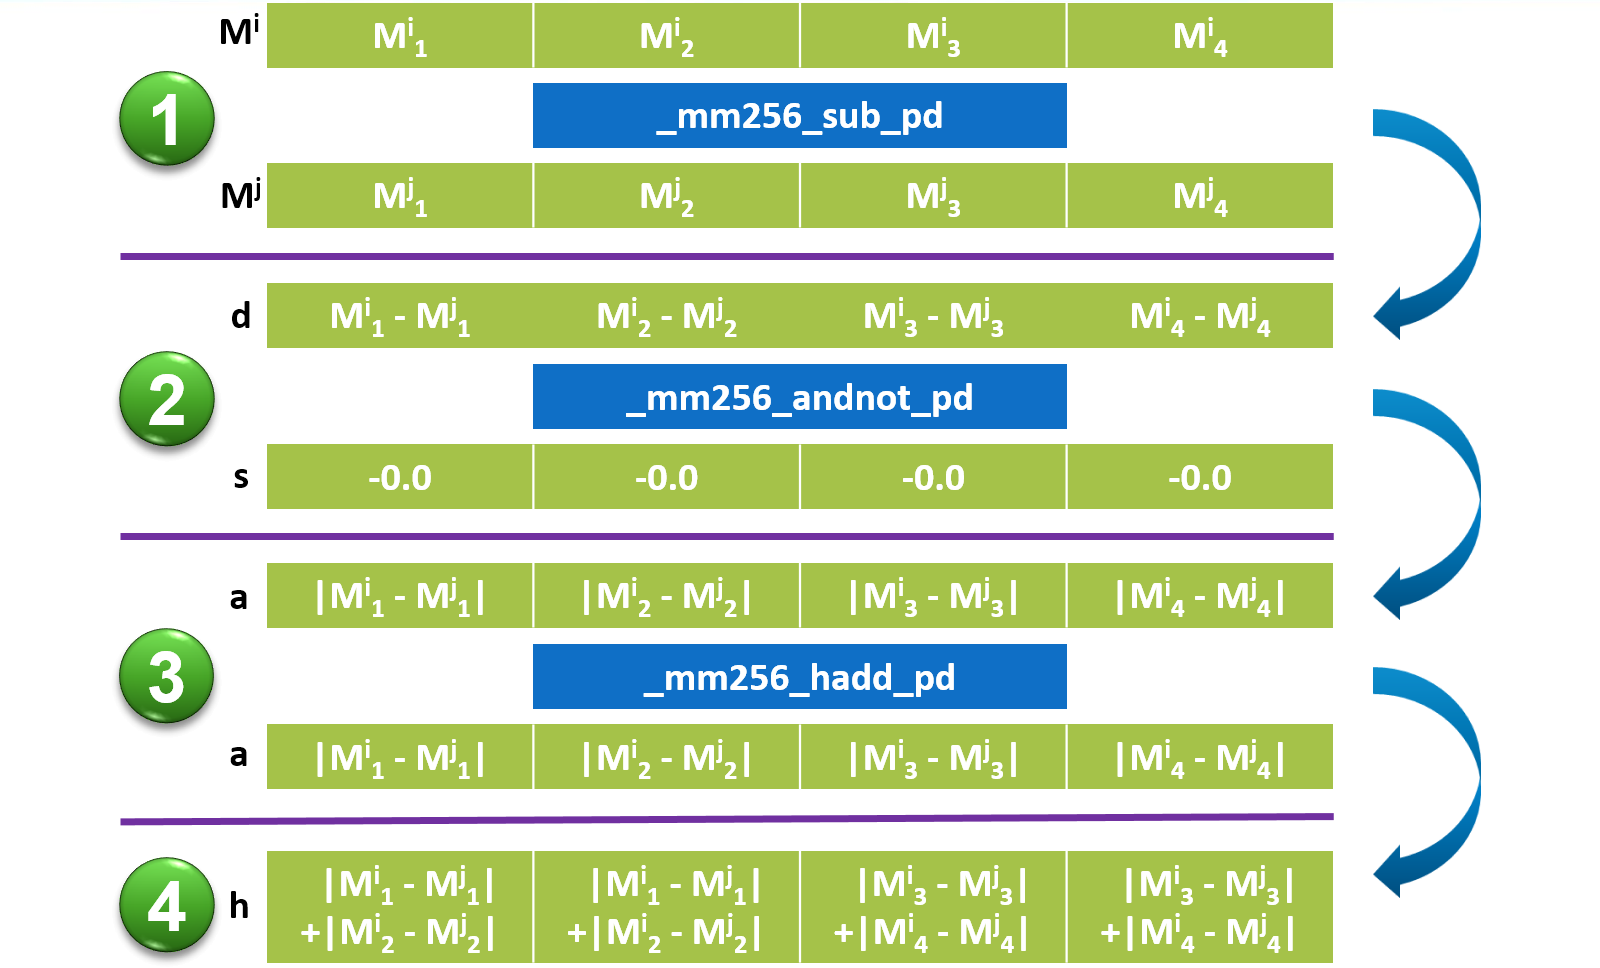
\includegraphics[width=\linewidth]{../usr/AVX.png}
\end{center}
\caption{AVX instructions used to compute USR or USRCAT scores.}
\label{AVX}
\end{figure}

Our daemon supports a query molecule in either SDF, MOL2, XYZ, PDB or PDBQT format in one single job. Sample files in these formats are provided in the USR@istar web page. The parser on the server side is achieved by the C++ API of OpenBabel v2.3.2 \cite{968}, while the parser on the client side is our in-house JavaScript code. Moreover, our client side user interface features our WebGL visualizer iview \cite{1366} to realize interactive visualization of high-score hits.

In the current implementation, no indexing or clustering has been done to accelerate searching. Supporting geometrical and functional clustering would be an exciting future direction.

\section{RESULTS}



\section{DISCUSSION}



\section{CONCLUSION}

Searching for compounds that resemble the shape of a given query molecule is a widely seen yet daunting problem in ligand-based virtual screening \cite{1332,1380,1281,1504,1502,1615} and macromolecular target prediction \cite{1407,1408,1402}. The USR-like methods \cite{1379,1338,1331} represent an entirely new class of non-superposition algorithms that effectively capture the molecular shape information independent of spatial position and orientation. These methods circumvent the requirement of structural alignment and show outstanding computational efficiency with respect to superposition-based methods \cite{1440,887,1439}.

In this study we have reviewed the traditional USR method \cite{1379} and its various extensions \cite{1333,1436,1437,1334,1335,1337,1338,1331,1407,1408,1675}, as well as their applications, both retrospective \cite{1332,1331} and prospective \cite{1505,1380,1281,1504,1502,1615}. We have highlighted the pros and cons of three web servers \cite{1436,1437,1408} which use USR variants as their underlying methods. Consequently, to address the existing constraints, we have designed our pragmatic implementation of USR \cite{1379} and USRCAT \cite{1331} on istar \cite{1362} and explained its methodological advancement in terms of functionality, usability, and efficiency.

First and foremost, our molecular database has been populated with more than 23 million small and diverse molecules that are collected from the ZINC database \cite{532,1178} and thus possibly commercially available to purchase for subsequent biological assays. We have also proposed to generate low-energy conformers that are likely to occur in nature. The reason why a molecular database should be populated with multiple conformers of each flexible compound is to reduce the possibility of missing compounds with similar shape to the query. We would use RDKit and the postprocessing algorithm suggested in \cite{1127} for the conformer generation task in the near future. The USR and USRCAT features of these 23 million compounds have been precalculated, which was a one-off exercise.

Second, we have estimated the storage size of all descriptors across the entire database, and suggested two approaches, i.e. preloading all descriptors at once and loading them chunk by chunk, and analyzed their theoretical execution time. Based on the time analysis, we have exploited three levels of parallelism, which map multiple jobs to multiple servers, multiple queries to multiple CPU cores, and multiple descriptors to multiple CPU registers, respectively, to fully utilize all available computational resources so as to accelerate job execution. Notably, we have described a novel AVX implementation of sum of absolute differences to calculate the USR or USRCAT scores between two moment vectors.

Moreover, our implementation of USR and USRCAT, denoted as USR@istar for short, supports a query molecule in SDF, MOL2, XYZ, PDB or PDBQT format. It also features our iview \cite{1366} WebGL visualizer to aid result interpretation in an interactive manner.

To benchmark USR@istar comprehensively, we selected 19 query molecules with different numbers of heavy atoms. To our expectation, sorting by USR or USRCAT score yielded different output, especially when the input ligand was large. From another perspective, when NRB was large, both methods did not manage to recover the query molecule in a different pose in the output because of the large conformational diversity implied by a large NRB. To our surprise, input file format impaired the classification of atoms into predefined pharmacophoric subsets, probably due to a bug in OpenBabel \cite{968}. We have also found that preloading database features boosted matching performance by four times.

We believe our USR@istar web service for ligand-based virtual screening purpose can perfectly supplement our idock@istar web service for structure-based virtual screening purpose. We suggest users try both services to reach a consensus. In the future we would provide a hybrid service that incorporates the advantages of idock@istar and USR@istar.

\section{AVAILABILITY}

USR@istar is free and open source under Apache License 2.0. It is available as a module of istar \cite{1362}. Our deployment of USR@istar is running at http://istar.cse.cuhk.edu.hk/usr. Sample query files are provided therein.

\section{ACKNOWLEDGEMENTS}

We gratefully acknowledge the Direct Grant from the Chinese University of Hong Kong, the GRF Grant (Project Reference 414413) from the Research Grants Council of Hong Kong SAR, the Inserm funding (P.J.B.), and the Medical Research Council for a Methodology Research Fellowship (Grant No. G0902106, awarded to P.J.B.).

\subsubsection{Conflict of interest statement.} None declared.
\newpage

\bibliographystyle{natbib} % Style BST file
\bibliography{../refworks} % Bibliography file (usually '*.bib' )

\end{document}
